\chapter{Methodologie und Systementwurf }

Hier werden über folgende Punkte diskutiert:

\begin{itemize}
	\item Die Entwicklungskonzeption, die wir während der Implementation der Anwendung benutzt haben, sowie die Tools, Technologien und Methodologien. 
	\item Überblick über Spring Boot und seine wichtigste  Funktionalitäten, die auch in dem Projekt angewendet sein werden. 
	\item Detaillierte Erklärung der Struktur und Design der Anwendung (Bsp: Anlyse-/Entwurfsdiagram) 
	\item Datenbanken, UI-Design und unterschiedliche Komponenten des Systems. 
	\item Wie Spring Boot die Entwicklung und Implementation der verschiedenen Module vereinfacht. 
\end{itemize}


\section{Entwurf und Konzeption}\index{Entwurf und Konzeption}

In der Softwareentwicklung spielen Entwurf und Konzeption eine entscheidende Rolle. Diese Phase des Entwicklungsprozesses befasst sich mit der Strukturierung und Planung von Systemen, bevor die eigentliche Implementierung beginnt. 

Ziel ist es, ein klares und verständliches Modell zu erstellen, das die Anforderungen und Funktionen eines Systems abbildet. In diesem Kapitel werden UML und einige Diagrammtypen vorgestellt.

\subsection{UML}\index{UML}

Die Unified Modeling Language (UML) ist ein wesentliches Werkzeug im Bereich Entwurf. UML ist eine standardisierte Modellierungssprache, die eine Vielzahl von Diagrammen bietet, um unterschiedliche Aspekte eines Systems darzustellen. Diese Diagramme helfen dabei, komplexe Systeme zu visualisieren, zu dokumentieren und zu kommunizieren \cite{UML:2023}. 

\subsection{Klassendiagramm}\index{Klassendiagramm}

\subsection{Use-Case Diagramme}\index{Use-Case Diagramme}


\section{Front-End Technologien}\index{Front-End Technologien}

Dieses Kapitel befasst sich mit Front-End-Technologien wie HTML, CSS, Typescript und Angular, die für die Erstellung interaktiver, reaktionsfähiger und visuell ansprechender Benutzeroberflächen in unserer E-Commerce-Anwendung unerlässlich sind.

\subsection{HTML/CSS}\index{HTML/CSS}

HTML\footnote{HyperText Markup Language} and CSS\footnote{Cascading Style Sheets} sind die grundlegenden Technologien zur Erstellung und Gestaltung von Webseiten. HTML liefert die Struktur und den Inhalt einer Webseite, während CSS für die visuelle Darstellung, Layout, Farben und Schriftarten, verwendet wird. Sie ermöglichen es optisch ansprechende und gut strukturierte Webseiten zu erstellen \cite{HTML/CSS:2024}.

\subsection{Typescript}\index{Typescript}

TypeScript\footnote{https://www.typescriptlang.org} ist eine stark typisierte Programmiersprache, die auf JavaScript aufbaut und statische Typdefinitionen hinzufügt. Sie soll die Entwicklung umfangreicher Anwendungen überschaubarer machen, indem sie es den Entwicklern ermöglicht, Fehler schon früh im Entwicklungsprozess zu erkennen, wodurch Fehler reduziert und die Codequalität verbessert werden. \cite{Typescript:2024}.\\
Die wichtigsten Vorteile von TypeScript sind:
\begin{itemize}
	\item \textbf{Statische Typisierung:} Die statische Typisierung  ermöglicht es Entwicklern, Variablentypen explizit zu definieren, was zu einer besseren Tooling-Unterstützung führt, z. B. bei der Code-Vervollständigung und beim Refactoring. Es hilft auch bei der Identifizierung von typbezogenen Fehlern während der Kompilierungszeit und nicht zur Laufzeit.
	\item \textbf{Wartbarkeit:} Durch die Hinzufügung von Typdefinitionen wird der Code selbstdokumentierender und leichter verständlich, was in großen Codebasen, in denen mehrere Entwickler zusammenarbeiten, entscheidend ist.
\end{itemize}
Durch die Wahl von TypeScript für das ShopNook-Projekt wurde es sichergestellt, dass das Frontend der Anwendung robust, wartbar und skalierbar ist und die hohen Anforderungen an eine professionelle E-Commerce-Plattform erfüllt.

\subsection{Angular}\index{Angular}

Angular\footnote{https://angular.io} ist ein Open-Source-Framework für Webanwendungen, das von Google entwickelt und gepflegt wird. Es wird für die Erstellung dynamischer, einseitiger Anwendungen (SPAs)\footnote{Single Page Application} mit TypeScript und HTML verwendet. Das Framework bietet eine robuste Plattform für die Entwicklung komplexer Anwendungen, indem es einen umfassenden Satz von Tools und Funktionen wie Datenbindung, Dependency Injection und eine modulare Architektur bietet \cite{Angular:2024}.\\
Eine der Hauptstärken von Angular ist seine komponentenbasierte Struktur, die es Entwicklern ermöglicht, wiederverwendbare UI-Komponenten zu erstellen, die die Wartbarkeit und Skalierbarkeit verbessern. Darüber hinaus bietet Angular leistungsstarke Funktionen wie reaktive Programmierung mit RxJS\footnote{https://rxjs.dev}, Zustandsverwaltung und ein reichhaltiges Ökosystem von Bibliotheken, was es zu einer idealen Wahl für Anwendungen auf Unternehmensebene macht.

\subsubsection{Komponentenbasierte Architektur}

Die komponentenbasierte Architektur von Angular gliedert die Anwendung in kleine, in sich geschlossene Einheiten, die als Komponenten bezeichnet werden. Jede Komponente kapselt einen bestimmten Teil der Benutzeroberfläche (UI) und die damit verbundene Logik \cite{Angular2:2024}.\\
Komponenten sind die wichtigsten Bausteine für Angular-Anwendungen. Wie es in der Abbildung \ref{a1} bezeichnet wurde besteht jede Komponente aus: 

\begin{figure} [h]
	\centering
	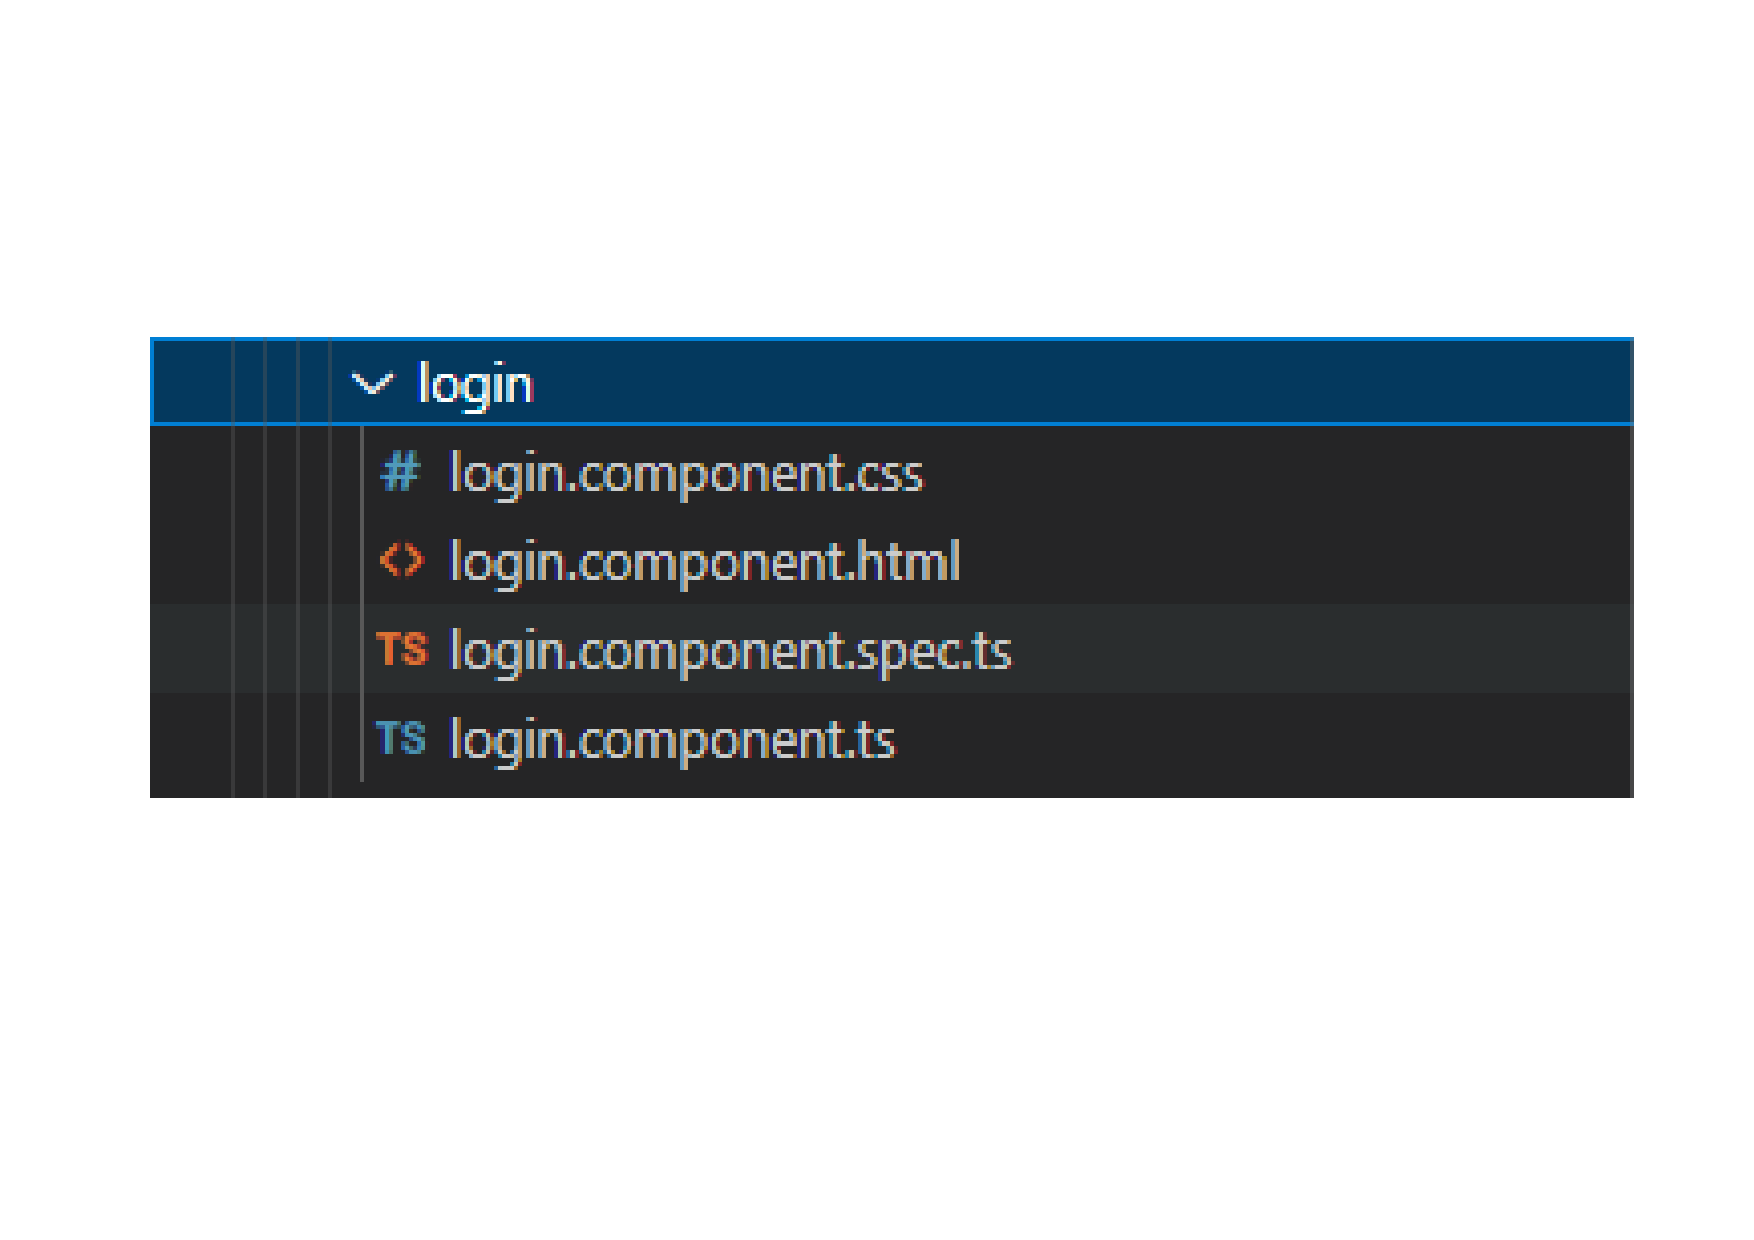
\includegraphics[scale=0.30]{images/Components.pdf}
	\caption{Beispielhafte Dateistruktur einer Angular-Anwendung mit verschiedenen Komponenten}
	\label{a1}
\end{figure}

\begin{itemize}
	\item einer Komponentendatei \texttt{<component-name>.component.ts}
	\item einer Vorlagedatei \texttt{<component-name>.component.html}
	\item einer CSS-Datei \texttt{<component-name>.component.css}
	\item Einer Datei mit Prüfvorschriften \texttt{<component-name>.component.spec.ts}
\end{itemize}


Dieser modulare Ansatz bringt mit sich mehrere Vorteile wie Wiederverwendbarkeit und Wartbarkeit.

\subsubsection{Single Page Application (SPA)}

Angular eignet sich besonders gut für die Erstellung von Single Page Applications (SPAs). In einer SPA lädt die gesamte Anwendung eine einzige HTML-Seite und aktualisiert den Inhalt dynamisch, wenn der Benutzer mit der Anwendung interagiert, ohne dass eine komplette Seite neu geladen werden muss \cite{Angular3:2024}. \\
Dieser Ansatz bietet mehrere Vorteile:
\begin{itemize}
	\item \textbf{Verbesserte Benutzerfreundlichkeit:} SPAs bieten eine reibungslosere und schnellere Benutzererfahrung, da nur die notwendigen Teile der Seite aktualisiert werden, anstatt die gesamte Seite neu zu laden.
	\item \textbf{Geringere Serverlast:} Sie entlasten den Server, da weniger Ganzseitenanfragen gestellt werden, was zu einer effizienteren Nutzung der Serverressourcen führt.
\end{itemize}

Durch die Nutzung der komponentenbasierten Architektur und der SPA-Funktionen von Angular kann die Anwendung ShopNook eine nahtlose und reaktionsschnelle Benutzererfahrung bieten, die für die Kundenbindung und -zufriedenheit entscheidend ist.


%\subsubsection{Document Object Model (DOM)}
\section{Back-End Technologien}\index{Back-End Technologien}

In diesem Kapitel werden Back-End-Technologien untersucht, wobei der Schwerpunkt auf Spring Boot liegt, um robuste, skalierbare und sichere serverseitige Logik und APIs für unsere E-Commerce-Anwendung zu erstellen.

\subsection{Java}\index{Java}

Java ist eine weit verbreitete Programmiersprache, die für ihre Plattformunabhängigkeit, Stabilität und umfassende Bibliotheken bekannt ist. Aufgrund ihrer Vielseitigkeit und Leistung wird Java häufig für die Entwicklung von Back-End-Anwendungen verwendet \cite{Java:2024}. In der E-Commerce-Anwendung (ShopNook) wird Java genutzt, um eine robuste und skalierbare serverseitige Logik zu gewährleisten.

\subsection{REST-API}\index{REST-API}

REST\footnote{Representational State Transfer} ist ein Architekturstil für die Entwicklung vernetzter Anwendungen. Er basiert auf einem zustandslosen, Client-Server- und cachefähigen Kommunikationsprotokoll, und in fast allen Fällen wird das HTTP-Protokoll verwendet. REST-APIs sind so konzipiert, dass sie einfach, leichtgewichtig und skalierbar sind, was sie zu einer beliebten Wahl für Webdienste macht \cite{REST:2024}.

\subsubsection{Einführung in REST}
Angelehnt an \cite{REST:2024} bieten REST-APIs eine Möglichkeit, über HTTP auf die Funktionalität und Daten einer Anwendung zuzugreifen. Sie folgen den Prinzipien von REST, die auf Ressourcen und deren Repräsentationen basieren. Jede Ressource wird durch eine eindeutige URI identifiziert und kann durch standardisierte HTTP-Methoden manipuliert werden:
\begin{itemize}
	\item GET: Abrufen von Ressourcen
	\item POST: Erstellen neuer Ressourcen
	\item PUT: Aktualisieren bestehender Ressourcen
	\item DELETE: Löschen von Ressourcen
\end{itemize}

REST-APIs sind also aufgrund ihrer Architektur und Funktionsweise weit verbreitet und bieten eine Reihe von Vorteilen:

\begin{itemize}
	\item \textbf{Skalierbarkeit:} Durch das stateless Design können REST-APIs leicht skaliert werden. Jeder HTTP-Request enthält alle notwendigen Informationen, um ihn zu verarbeiten, ohne dass der Server den vorherigen Zustand kennen muss.
	\item \textbf{Flexibilität:} REST-APIs sind flexibel und können mit verschiedenen Datenformaten arbeiten. JSON ist das gebräuchlichste Format, da es leichtgewichtig und gut lesbar ist.
	\item \textbf{Interoperabilität:\footnote{Interoperabilität ist die Fähigkeit verschiedener Systeme oder Software, zusammenzuarbeiten und Informationen nahtlos auszutauschen\cite{wiki:listing}.}} REST-APIs nutzen standardisierte HTTP-Methoden, was ihre Interoperabilität mit verschiedenen Clients und Plattformen gewährleistet.
	\item \textbf{Leichte Integration:} REST-APIs lassen sich leicht in bestehende Systeme integrieren, da sie auf bekannten Webstandards basieren.
\end{itemize}

Um die Sicherheit von REST-APIs in der ShopNook-Plattform weiter zu gewährleisten, spielt die Implementierung von HTTPS in Kombination mit SSL/TLS eine entscheidende Rolle, da diese Technologien eine sichere und verschlüsselte Kommunikation zwischen dem Client und dem Server ermöglichen.

\subsection{HTTPS und SSL/TLS}

HTTPS ist die sichere Version von HTTP, dem Protokoll, über das die Daten zwischen dem Browser des Kunden und der Website, mit der er verbunden ist, gesendet werden. Das „S“ am Ende von HTTPS steht für „Secure“, was bedeutet, dass die gesamte Kommunikation zwischen dem Kunden und dem Server verschlüsselt ist \cite{HTTPS:2024}.\\
SSL/TLS sind allerdings Verschlüsselungsprotokolle, die eine sichere Kommunikation über ein Computernetz ermöglichen. SSL war das ursprüngliche Protokoll, aber es wurde zugunsten von TLS, das sicherer und effizienter ist, veraltet \cite{SSL/TLS:2023}. Diese Protokolle bieten mehrere wichtige Sicherheitsfunktionen, die im Folgenden näher erläutert werden:

\begin{itemize}
	\item \textbf{Verschlüsselung der Daten:} SSL und TLS verschlüsseln die zwischen dem Client und dem Server übertragenen Daten und stellt sicher, dass die Daten, selbst wenn sie abgefangen werden, nicht von Unbefugten gelesen werden können.
	\item \textbf{Server-Authentifizierung:} Diese Protokolle überprüfen auch die Identität des Servers und stellen sicher, dass die Clients mit einem legitimen Server und nicht mit einem Betrüger kommunizieren.
	\item \textbf{Datenintegrität:} Sie bieten auch Datenintegrität, indem es sicherstellt, dass die Daten während der Übertragung nicht manipuliert wurden.
\end{itemize}
In der Anwendung wurde eine HTTPS Konfiguration (siehe \ref{HTTPS-Config}) erstellt, um eine sichere Kommunikation zwischen Clients und dem Server zu gewährleisten. Dazu wurde der Server so eingestellt, dass er auf Port 8443 auf HTTPS-Datenverkehr wartet. Der Konfigurationsprozess beinhaltete die Aktivierung der SSL-Unterstützung, die für die Verschlüsselung der über das Netzwerk ausgetauschten Daten unerlässlich ist.\\
Wir haben eine Keystore-Datei im PKCS12-Format \textbf{(shopnook-keystore.p12)} verwendet, in der die für die Verschlüsselung erforderlichen SSL/TLS-Zertifikate sicher gespeichert sind. Der Keystore ist durch ein Passwort geschützt \textbf{(server.ssl.key-store-password=secret)}, so dass der Zugriff auf die kryptografischen Schlüssel nur autorisierten Prozessen vorbehalten ist.\\
Innerhalb des Schlüsselspeichers wird das Zertifikat durch den Alias \textbf{shopnook} identifiziert, auf den in der Konfiguration verwiesen wird, um die SSL-Vorgänge des Servers mit dem richtigen Zertifikat zu verknüpfen. Diese Einrichtung stellt sicher, dass alle zwischen dem Client und dem Server übertragenen Daten verschlüsselt werden, was einen robusten Schutz gegen Abhör- und Man-in-the-Middle-Angriffe bietet.\\
Darüber hinaus ermöglicht die Konfiguration eine einfache Anpassung an unterschiedliche Umgebungen. So kann beispielsweise der Port der Anwendung je nach Einsatzumgebung geändert werden, indem die Eigenschaft \textbf{server.port} angepasst wird. Für die QA-Demo-Umgebung ist der Port auf \textbf{9898} eingestellt, der durch Umschalten der Kommentarzeilen aktiviert werden kann.\\
Durch die sorgfältige Konfiguration dieser SSL-Einstellungen stellen wir sicher, dass ShopNook den Industriestandards für Sicherheit entspricht.\newpage

\begin{lstlisting}[language=, caption={Implementierung von HTTPS und SSL Konfiguration}\label{HTTPS-Config}]
	#####
	#
	# HTTPS configuration
	#
	#####
	#Define the web server's listening port for HTTPS traffic
	server.port=8443 
	
	#QA Demo Port
	#server.port=9898
	
	#Activate SSL support to secure the application with HTTPS
	server.ssl.enabled=true
	
	#Specify the key alias used within the keystore for SSL
	server.ssl.key-alias=shopnook
	
	#Keystore path
	server.ssl.key-store=classpath:shopnook-keystore.p12
	
	#Password to unlock the keystore and access the SSL keys
	server.ssl.key-store-password=secret
	
	#format of the keystore file
	server.ssl.key-store-type=PKCS12
\end{lstlisting}



Durch die Implementierung von HTTPS mit SSL/TLS hält sich ShopNook an die Industriestandards für Datensicherheit, um seine Nutzer zu schützen und das Vertrauen zu erhalten. Dies ist ein entscheidender Aspekt des Backends der Anwendung, insbesondere für die Wahrung der Vertraulichkeit und Integrität sensibler Daten bei Transaktionen.

\subsection{Spring Boot}\index{Spring Boot}

Spring Boot ist ein Framework, das auf dem Spring Framework aufbaut und speziell entwickelt wurde, um schnelle, effiziente und skalierbare Anwendungen zu erstellen. Es bietet eine Vielzahl von Features, die den Entwicklungsprozess beschleunigen und vereinfachen, insbesondere für Java-basierte Webanwendungen und Microservices.

\subsubsection{Warum wurde Spring Boot ausgewählt ?}
Spring Boot wurde aufgrund der breiten Unterstützung in der Entwicklergemeinde ausgewählt. Hier sind einige der Hauptgründe:
\begin{itemize}
	\item \textbf{Produktivität:} Das Framework ermöglicht es auf das Schreiben von Geschäftslogik zu konzentrieren, anstatt sich um die Konfiguration von Technologien zu kümmern.
	\item \textbf{Microservices:} Es eignet sich hervorragend für die Entwicklung von Microservices-Architekturen, indem es Server wie Tomcat bietet, sodass die Anwendungen ohne externen Server laufen können.
	\item \textbf{Integration:} Es lässt sich nahtlos in andere Spring-Projekte und eine Vielzahl von Datenbanken integrieren.
\end{itemize}
Das Framework bietet auch viele Funktionalitäten, die es von anderen abheben, es hat viele weitere Vorteile, die hier genannt werden:

\begin{itemize}
	\item \textbf{Auto-Konfiguration:} Die Autokonfigurationsfunktion von Spring Boot konfiguriert Ihre Anwendung automatisch anhand der Abhängigkeiten, die Sie dem Projekt hinzugefügt haben. Dadurch wird die Notwendigkeit einer manuellen Konfiguration minimiert und die Entwicklung beschleunigt.
	\item \textbf{Eigenständige Anwendungen:} Spring Boot-Anwendungen können als eigenständige Java-Anwendungen verpackt werden, was die Bereitstellung einfacher und konsistenter macht.
	\item \textbf{Produktionstaugliche Funktionen:} Das Framework umfasst zahlreiche produktionsreife Funktionen wie Zustandsprüfungen, Metriken und externalisierte Konfiguration.	
\end{itemize}

\subsubsection{Wie funktionniert Spring Boot ?}

\begin{enumerate}
	\item \textbf{Initial Setup:} Mit Spring Initializr kann man schnell ein neues Spring Boot-Projekt mit allen erforderlichen Abhängigkeiten und Konfigurationen initialisieren.
	\item \textbf{Main Application Class:} Jede Spring Boot-Anwendung hat eine Hauptklasse, die mit @SpringBootApplication annotiert ist. Diese Annotation ist eine Kombination aus @Configuration, @EnableAutoConfiguration und @ComponentScan.
	\begin{lstlisting}[language=Java, caption={Main-Application-Class-Implementierung in Java}\label{mainClass.java}]
@SpringBootApplication
public class SpringBootEcommerceApplication {	
	public static void main(String[] args) {
		SpringApplication.run(SpringBootEcommerceApplication.class, args);
	}
}		
	\end{lstlisting}
	\item \textbf{Application Properties:} Spring Boot ermöglicht eine einfache Konfiguration durch application.properties-Datei. Dadurch wird die Konfiguration externalisiert, was die Verwaltung verschiedener Umgebungen erleichtert.
	\begin{lstlisting}[language=Java, caption={Implementierung von Application.properties Datei}\label{Application.properties}]
spring.datasource.driver-class-name=com.mysql.cj.jdbc.Driver
spring.datasource.url=jdbc:mysql://localhost:3306/full-stack-ecommerce?
useSSL=false&useUnicode=yes&characterEncoding=UTF-8&allowPublicKeyRetrieval=
true&serverTimezone=UTC
spring.datasource.username=username
spring.datasource.password=password
spring.jpa.properties.hibernate.dialect=org.hibernate.dialect.MySQL8Dialect
spring.data.rest.base-path=/api
	\end{lstlisting}
\end{enumerate}

\subsubsection{Spring Security}

Spring Security ist ein robustes und anpassungsfähiges Framework, das für die Authentifizierung und Zugriffskontrolle entwickelt wurde und sich zum Standard für die Absicherung von mit Spring erstellten Anwendungen entwickelt hat.

Spring Security ist ein Framework, das sowohl die Authentifizierung als auch die Autorisierung von Java-Anwendungen übernimmt. Seine Stärke liegt in der Flexibilität, die es erlaubt, es leicht zu erweitern, um spezifische Anforderungen zu erfüllen.

Das Framework bietet eine Reihe von Funktionen, darunter umfassende Unterstützung für Authentifizierung und Autorisierung, Schutz vor verschiedenen Angriffen wie Session Fixation, Clickjacking und Cross-Site Request Forgery, Integration mit der Servlet API und optionale Kompatibilität mit Spring Web MVC \cite{Spring-Security:o.J}.

Zum Schutz der Endpunkte für Kundenbestellungen wurde Spring Security mit OAuth2-Authentifizierung implementiert, wobei JWT zur Gewährleistung eines sicheren Zugriffs verwendet wird. Die Einrichtung umfasste die Konfiguration von CORS zur Verwaltung von Herkunftsübergreifenden Anfragen und die Anpassung von Sicherheitseinstellungen wie die Deaktivierung des CSRF-Schutzes und die Handhabung der Inhaltsaushandlung. Dieser Ansatz gewährleistet robuste Sicherheit, während er verschiedene Inhaltstypen unterstützt und die gemeinsame Nutzung von Ressourcen über verschiedene Ursprünge hinweg effektiv handhabt.

\subsection{Stripe API}

\section{Datenbankstruktur}\index{Datenbankstruktur}
In diesem Abschnitt wird die Datenbankstruktur der Webanwendung untersucht, um ein umfassendes Verständnis für die Organisation, den Zugriff und die Verwaltung der Daten zu vermitteln. Der Schwerpunkt liegt auf dem relationalen Datenbankmodell und den spezifischen Technologien und Frameworks, die zur Handhabung der Datenpersistenz und der Transaktionen verwendet werden. Dabei wird MySQL als das gewählte Datenbanksystem zusammen mit Spring Data JPA für eine nahtlose Dateninteraktion untersucht. In den folgenden Unterabschnitten werden diese Aspekte im Detail behandelt, wobei relationale Datenbanken, die Auswahl von MySQL, Datenpersistenz und Transaktionsmanagement sowie die Integration von MySQL mit Spring Boot behandelt werden.
\subsection{Übersicht über relationale Datenbanken und Auswahl von MySQL}
Die Daten in einer relationalen Datenbank sind in Tabellen mit Spalten und Zeilen organisiert, und auch die Primär- und Fremdschlüssel werden verwendet, um die Beziehungen zwischen den Tabellen herzustellen. Dieser Ansatz ist ideal für E-Commerce-Anwendungen, da er komplexe Abfragen und aussagekräftige Daten verarbeiten kann. Produktlieferungen, Auftragstransaktionen und Kundendaten werden alle ordnungsgemäß verwaltet. Die Möglichkeit, Tabellen zu verknüpfen, erleichtert umfassende Analysen, einschließlich der Nachverfolgung von Kaufdatensätzen und der Bestandskontrolle, während die Einhaltung von ACID-Eigenschaften eine zuverlässige Transaktionsverarbeitung gewährleistet, die für die Auftragsabwicklung und das Zahlungsmanagement entscheidend ist. Relationale Datenbanken wie MySQL bieten die Robustheit und Konsistenz, die für einen sicheren und produktiven Online-Shopping-Betrieb erforderlich sind \cite{IBM:o.J}.

\subsection{Datenbankschemaentwurf mit Spring Data JPA}
Ziel dieses Abschnitts ist es, zu erörtern, wie Spring Data JPA den Entwurf und die Verwaltung von Datenbankschemata vereinfacht. Es wird gezeigt, wie Spring Data JPA es Entwicklern ermöglicht, Entitäten und Beziehungen innerhalb eines Datenbankschemas abzubilden und zu verwalten, und wie es die Komplexität des Datenzugriffs durch seine Repository-Schicht abstrahiert.

Spring Data JPA vereinfacht den Entwurf von Datenbankschemata, indem es Entwicklern ermöglicht, Java-Klassen mithilfe von Annotationen wie @Entity, @Id und @OneToMany auf Datenbanktabellen abzubilden. Diese Annotationen übernehmen automatisch die Schemaerstellung und -verwaltung und stellen sicher, dass die Datenbankstruktur mit dem Domänenmodell der Anwendung übereinstimmt \cite{Docs-Spring:o.J, Baeldung:o.J}.

Die Repository-Schicht in Spring Data JPA abstrahiert die Komplexität des Datenzugriffs und bietet integrierte CRUD-Operationen über Schnittstellen wie JpaRepository. Dies macht manuelle SQL-Abfragen überflüssig und rationalisiert die Datenbankinteraktionen, so dass sich die Entwickler auf die Geschäftslogik konzentrieren können \cite{Docs-Spring-JPA-Repo:o.J, Docs-Spring-JPA-QueryMethods:o.J}.

\subsection{Datenpersistenz und Transaktionen}
In diesem Abschnitt wird erläutert, wie Spring Boot und Hibernate die Datenpersistenz handhaben. Der Schwerpunkt liegt dabei auf CRUD-Operationen, der Rolle des EntityManagers und der Interaktion des Hibernate ORM mit MySQL.

CRUD-Operationen werden mit Spring Boot und Hibernate verwaltet. Der EntityManager ist in diesem Prozess von zentraler Bedeutung und ermöglicht das Erstellen, Abrufen, Aktualisieren und Löschen von Entitäten. Er verwaltet auch den Lebenszyklus von Entitäten innerhalb von Transaktionen und stellt sicher, dass Änderungen bei Bedarf ordnungsgemäß übertragen oder zurückgenommen werden  \cite{Baeldung-EntityManager:2024}.


Hibernate ORM wird verwendet, um Java-Objekte auf Datenbanktabellen abzubilden, was die Interaktion mit der MySQL-Datenbank vereinfacht. Dieses ORM-Framework macht manuelles SQL überflüssig und bietet einen objektorientierten Ansatz für Datenbankoperationen \cite{Hibernate:o.J}.


\subsection{MySQL-Workbench und SQL}
In diesem Abschnitt wird die MySQL Workbench als Werkzeug für den Entwurf und die Verwaltung von Datenbanken und SQL als Sprache für die Erstellung von Abfragen und die Verwaltung der Datenbank vorgestellt.

MySQL Workbench wurde zur Visualisierung des Datenbankschemas eingesetzt und ermöglichte eine intuitive Gestaltung und Verwaltung der Datenbankstrukturen. Sie erleichterte die Erstellung und Änderung von Tabellen, Beziehungen und Indizes. Darüber hinaus wurde SQL verwendet, um Abfragen für Tests und die Datenbankverwaltung auszuführen, einschließlich Aufgaben wie Datenmanipulation und Schemaaktualisierungen \cite{mySQL:o.J}.

\subsection{Datenbankverbindung und -konfiguration in Spring Boot}
In diesem Abschnitt wird erläutert, wie die Datenbank innerhalb der Spring Boot-Anwendung verbunden und konfiguriert wird.

Die Datenbankverbindung wird in der Datei \texttt{application.properties} konfiguriert. Zu den wichtigsten Eigenschaften gehören die JDBC-URL, der Name der Treiberklasse und die Anmeldeinformationen, wie in \hyperref[Application.properties]{Listing~2.2} dargestellt.

\section{Authentifizierungs- und Autorisierungsprotokolle}\index{Authentifizierungs- und Autorisierungsprotokolle}

In der modernen digitalen Landschaft ist die Gewährleistung eines sicheren Zugriffs auf Ressourcen von entscheidender Bedeutung. In diesem Abschnitt werden die wichtigsten Protokolle und Standards zur Verwaltung der Benutzerauthentifizierung und -autorisierung untersucht, darunter JWT, OAuth2 und OpenID Connect.

\subsection{Okta}
Okta verbindet Benutzer mit jeder Anwendung über alle Geräte hinweg. Es ist ein Cloud-basierter Identitätsmanagement-Service, der mit verschiedenen lokalen Systemen kompatibel ist. Okta bietet der IT-Abteilung die Möglichkeit, den Zugriff auf Anwendungen und Geräte über eine sichere, zuverlässige und gut geprüfte Cloud-Plattform zu verwalten, mit einer tiefen Integration in lokale Systeme und Verzeichnisse.

Okta bietet Funktionen wie Provisioning, Single Sign-On (SSO), Active Directory (AD) und LDAP-Integration, zentrales Nutzer-Deprovisioning, Multi-Faktor-Authentifizierung (MFA), mobiles Identitätsmanagement und anpassbare Sicherheitsrichtlinien. Diese Funktionen werden durch das Okta Integration Network (OIN) vereinheitlicht, das umfangreiche Integrationsoptionen bietet und SSO für alle Anwendungen ermöglicht, die Ihre Benutzer benötigen\cite{Okta:o.J}.

\subsection{JWT}

JWT ist ein offener Standard (RFC 7519) für die sichere Übertragung von Informationen in Form eines JSON-Objekts. Diese Informationen sind aufgrund der digitalen Unterzeichnung überprüfbar und vertrauenswürdig. JWTs können mit einem geheimen Schlüssel mit HMAC oder mit einem öffentlichen/privaten Schlüsselpaar mit RSA oder ECDSA signiert werden. Hier sind einige Situationen, in denen JSON-Web-Token von Vorteil sind:

\begin{itemize}
	\item \textbf{Autorisierung:}  JWTs werden in der Regel zur Authentifizierung verwendet. Nach der Anmeldung enthält jede Anfrage das JWT, das den Zugriff auf autorisierte Routen, Dienste und Ressourcen ermöglicht.
	\item \textbf{Informationsaustausch:} Mit JWTs werden Informationen sicher zwischen Parteien übertragen. Signierte JWTs bestätigen die Identität des Absenders und stellen sicher, dass der Inhalt unverändert bleibt, da die Signatur sowohl aus der Kopfzeile als auch aus der Nutzlast abgeleitet wird\cite{JWT:o.J}.
\end{itemize}

\subsection{OAuth2}
OAuth 2.0, kurz für „Open Authorization“, ist ein Standard, der es einer Website oder Anwendung ermöglicht, im Namen eines Benutzers auf Ressourcen anderer Webanwendungen zuzugreifen. Er löste 2012 OAuth 1.0 ab und hat sich seitdem zum Industriestandard für die Online-Autorisierung entwickelt. OAuth 2.0 erleichtert den autorisierten Zugriff und schränkt gleichzeitig die Aktionen ein, die eine Client-Anwendung für den Benutzer auf Ressourcen durchführen kann, ohne die Anmeldedaten des Benutzers preiszugeben\cite{OAuth2:o.J}.

\subsection{OpenID Connect}
OpenID Connect ist ein Authentifizierungsprotokoll, das auf dem OAuth 2.0 Framework (IETF RFC 6749 und 6750) aufbaut. Es rationalisiert die Überprüfung der Benutzeridentität, indem es die von einem Autorisierungsserver durchgeführte Authentifizierung nutzt und Benutzerprofilinformationen in einer RESTful und interoperablen Weise bereitstellt.

OpenID Connect fördert ein Internet-Identitäts-Ökosystem durch einfache Integration, Sicherheits- und Datenschutzfunktionen, breite Client- und Gerätehilfe und die Möglichkeit für jede Einrichtung, als OpenID Provider (OP) zu agieren\cite{OpenId:o.J}.


\section{Entwicklungsumgebung und Versionskontrolle}\index{Entwicklungsumgebung und Versionskontrolle}
In diesem Abschnitt werden die integrierten Entwicklungsumgebungen (IDEs) und Versionskontrollsysteme beschrieben, die im Rahmen des Projekts eingesetzt wurden. Er bietet einen Überblick über die für die Entwicklung ausgewählten IDEs und die Versionskontrollwerkzeuge, die zur effektiven Verwaltung von Codeänderungen eingesetzt wurden.
\subsection{Entwicklungsumgebung}
Dieser Unterabschnitt beschreibt die im Projekt verwendeten Entwicklungsumgebungen, wobei der Schwerpunkt auf IntelliJ IDEA und Visual Studio Code (VS Code) liegt. Er hebt die Funktionen und Vorteile der einzelnen IDEs bei der Unterstützung des Entwicklungsprozesses und der Steigerung der Produktivität hervor.

\subsubsection{IntelliJ IDEA}

IntelliJ IDEA ist bekannt für seinen leistungsstarken Code-Editor, der sich durch eine umfassende Anfangsindizierung beim Verstehen und Verwalten von Code auszeichnet. Diese Funktion ermöglicht es ihm, Fehler in Echtzeit zu erkennen, kontextbezogene Vorschläge zur Code-Vervollständigung anzubieten und sicheres Code-Refactoring durchzuführen, neben anderen Funktionen. Es ist mit einer umfangreichen Suite integrierter Entwicklerwerkzeuge ausgestattet und bietet robuste Unterstützung für verschiedene Spring-Frameworks sowohl in Java als auch in Kotlin. Dazu gehören Spring MVC, Spring Boot, Spring Integration, Spring Security und Spring Cloud. Zu den bemerkenswerten Vorteilen gehören intelligente Codierungshilfe, sofortige Navigation innerhalb des Spring-Codes, integrierte Entwicklungswerkzeuge und erweiterte Visualisierungsfunktionen \cite{Jetbrains:o.J}.


\subsubsection{Visual Studio Code}

 Visual Studio Code ist ein vielseitiger und effizienter Quellcode-Editor, der mit Windows, macOS und Linux kompatibel ist. Er bietet native Unterstützung für JavaScript, TypeScript und Node.js und verfügt über eine breite Palette von Erweiterungen für weitere Sprachen und Plattformen \cite{visual-studio:o.J}.

Da die Front-End-Entwicklung Angular, ein auf TypeScript basierendes Framework, nutzt, wurde Visual Studio Code als Entwicklungsumgebung gewählt. Die starke native Unterstützung für TypeScript erleichtert die effiziente und optimierte Projektentwicklung und macht zusätzliche Erweiterungen überflüssig. \cite{visualstudio-angular:o.J}.

\subsection{Versionskontrolle}
In diesem Unterabschnitt werden die im Projekt eingesetzten Versionskontrollsysteme beschrieben, wobei der Schwerpunkt auf Git und GitHub liegt. Es wird erläutert, wie diese Tools die Codeverwaltung, die Zusammenarbeit und die Verfolgung von Änderungen während des gesamten Entwicklungsprozesses erleichtert haben.
\subsubsection{Git}
Git ist ein kostenloses und quelloffenes, verteiltes Versionskontrollsystem, das entwickelt wurde, um Projekte jeder Größe schnell und effizient zu verwalten. Es hat einen minimalen Platzbedarf und liefert eine außergewöhnlich schnelle Leistung. Git übertrifft herkömmliche SCM-Tools wie Subversion, CVS, Perforce und ClearCase mit Funktionen wie kostengünstiger lokaler Verzweigung, benutzerfreundlichen Staging-Bereichen und flexiblen Arbeitsabläufen.

Eines der herausragenden Merkmale von Git ist sein Verzweigungsmodell, das es von fast allen anderen SCM-Tools unterscheidet. Git ermöglicht und fördert die Erstellung mehrerer lokaler Zweige, von denen jeder unabhängig funktionieren kann. Das Erstellen, Zusammenführen und Löschen von Zweigen geht schnell, nahtlos vonstatten und dauert oft nur Sekunden  \cite{git-scmr:o.J}.

\subsubsection{GitHub}
GitHub ist eine cloudbasierte Plattform zum Speichern, Freigeben und gemeinsamen Bearbeiten von Code. Die von Git unterstützten Kollaborationsfunktionen von GitHub ermöglichen es uns:

\begin{itemize}
	\item Projekte zu präsentieren oder zu verbreiten.
	\item Verfolgen und Verwalten von Codeänderungen im Laufe der Zeit.
	\item Andere einladen, den Code zu überprüfen und Verbesserungen vorzuschlagen.
	\item Zusammenarbeit an Projekten ohne das Risiko, dass unbeabsichtigte Änderungen die Arbeit der anderen beeinträchtigen, bis die Änderungen integriert werden können.  \cite{github:o.J}.
\end{itemize} 














